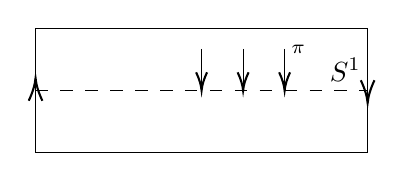
\begin{tikzpicture}[x=0.75pt,y=0.75pt,yscale=-1,xscale=1]
    %uncomment if require: \path (0,300); %set diagram left start at 0, and has height of 300
    
    %Straight Lines [id:da575614681710741] 
    \draw    (150,90) -- (310,90) ;
    %Straight Lines [id:da7355250432830472] 
    \draw    (150,150) -- (310,150) ;
    %Straight Lines [id:da425921249207598] 
    \draw  [dash pattern={on 4.5pt off 4.5pt}]  (150,120) -- (310,120) ;
    %Straight Lines [id:da15541437714065776] 
    \draw    (150,150) -- (150,90) ;
    \draw [shift={(150,114)}, rotate = 90] [color={rgb, 255:red, 0; green, 0; blue, 0 }  ][line width=0.75]    (10.93,-3.29) .. controls (6.95,-1.4) and (3.31,-0.3) .. (0,0) .. controls (3.31,0.3) and (6.95,1.4) .. (10.93,3.29)   ;
    %Straight Lines [id:da40082781733479333] 
    \draw    (310,90) -- (310,150) ;
    \draw [shift={(310,126)}, rotate = 270] [color={rgb, 255:red, 0; green, 0; blue, 0 }  ][line width=0.75]    (10.93,-3.29) .. controls (6.95,-1.4) and (3.31,-0.3) .. (0,0) .. controls (3.31,0.3) and (6.95,1.4) .. (10.93,3.29)   ;
    %Straight Lines [id:da6754846896588976] 
    \draw    (270,100) -- (270,118) ;
    \draw [shift={(270,120)}, rotate = 270] [color={rgb, 255:red, 0; green, 0; blue, 0 }  ][line width=0.75]    (8.74,-2.63) .. controls (5.56,-1.12) and (2.65,-0.24) .. (0,0) .. controls (2.65,0.24) and (5.56,1.12) .. (8.74,2.63)   ;
    %Straight Lines [id:da23038618406097078] 
    \draw    (250,100) -- (250,118) ;
    \draw [shift={(250,120)}, rotate = 270] [color={rgb, 255:red, 0; green, 0; blue, 0 }  ][line width=0.75]    (8.74,-2.63) .. controls (5.56,-1.12) and (2.65,-0.24) .. (0,0) .. controls (2.65,0.24) and (5.56,1.12) .. (8.74,2.63)   ;
    %Straight Lines [id:da41624213159172174] 
    \draw    (230,100) -- (230,118) ;
    \draw [shift={(230,120)}, rotate = 270] [color={rgb, 255:red, 0; green, 0; blue, 0 }  ][line width=0.75]    (8.74,-2.63) .. controls (5.56,-1.12) and (2.65,-0.24) .. (0,0) .. controls (2.65,0.24) and (5.56,1.12) .. (8.74,2.63)   ;
    
    % Text Node
    \draw (272,100) node [anchor=west] [inner sep=0.75pt]  [font=\scriptsize] [align=left] {$\displaystyle \pi $};
    % Text Node
    \draw (308,117) node [anchor=south east] [inner sep=0.75pt]   [align=left] {$\displaystyle S^{1}$};
    
    
\end{tikzpicture}